\documentclass[a4paper,12pt]{article}
\usepackage[hmargin=2.5cm,vmargin=2.5cm]{geometry}

\usepackage[utf8]{inputenc}   % le fichier .tex est en UTF-8     
\usepackage[francais]{babel}  %typo française                    
\usepackage[T1]{fontenc}      % encodage des fonts latex         
\usepackage{lmodern}                                             
\usepackage{microtype}        % typo supplémentaires             
\usepackage{booktabs}

\usepackage{multirow}  %  pour des tableaux multilignes/multicolonnes

\usepackage{graphicx} %inclusion de graphiques

\usepackage{hyperref} % liens dans le pdf
\hypersetup{%
  pdftitle={Title},
  pdfauthor={Author1, Author2},
  pdfkeywords={keywords}
  pdfsubject={article},
  colorlinks=true,
  linkcolor=black,
  urlcolor=black,
  citecolor=black
}


\begin{document}

   \begin{figure}[t]
     \centering
     \begin{tabular}{cc}
       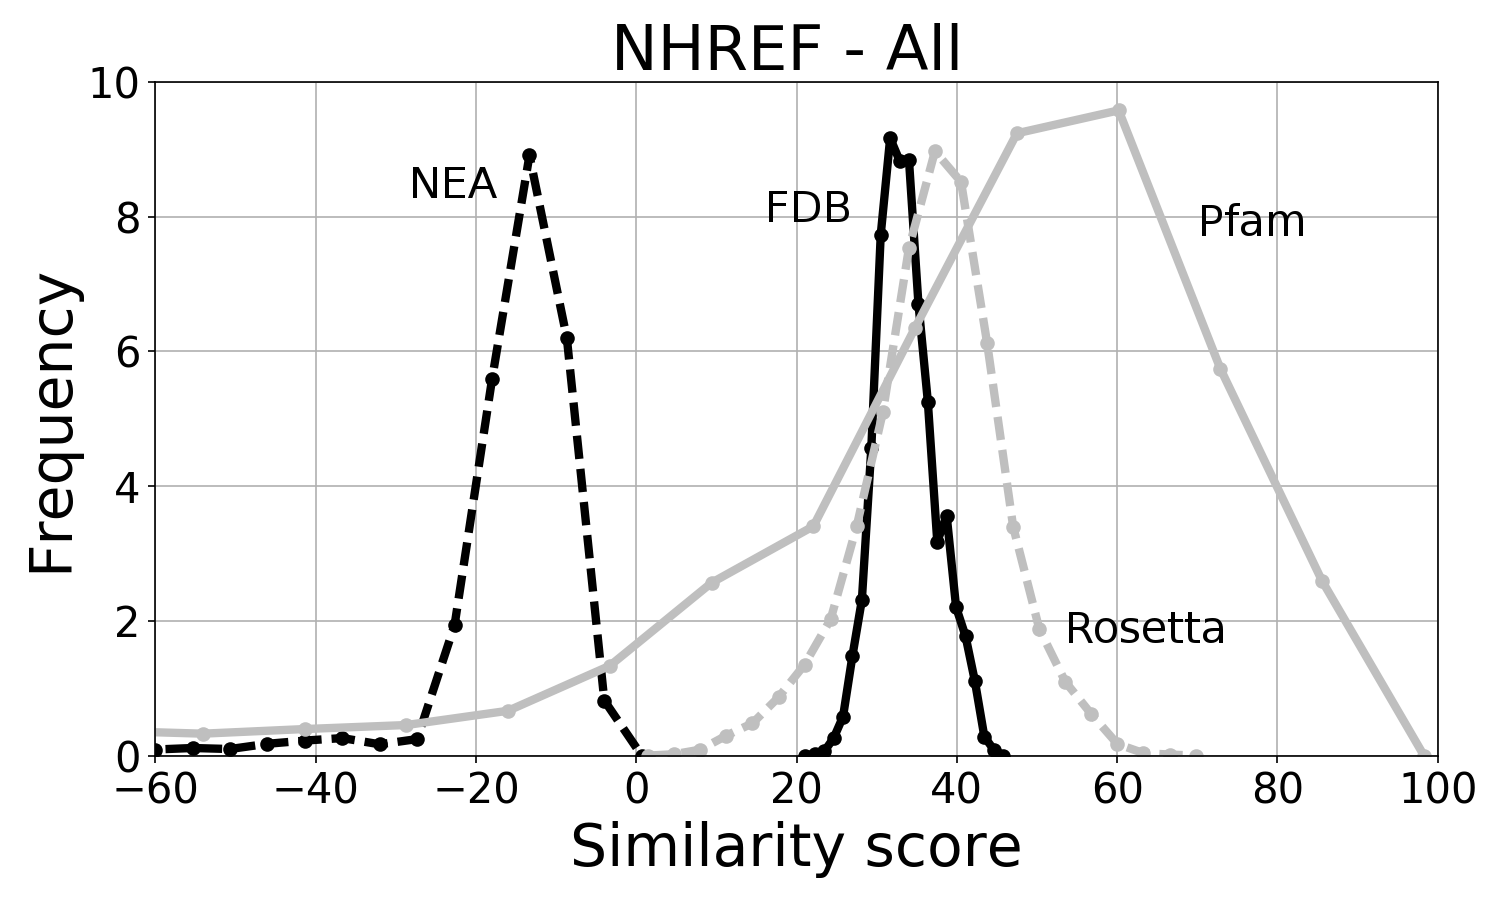
\includegraphics[width=8.4cm]{rapport/resultats/PDZ/graphe/exactGB/1G9O_simil_cut.png} &
       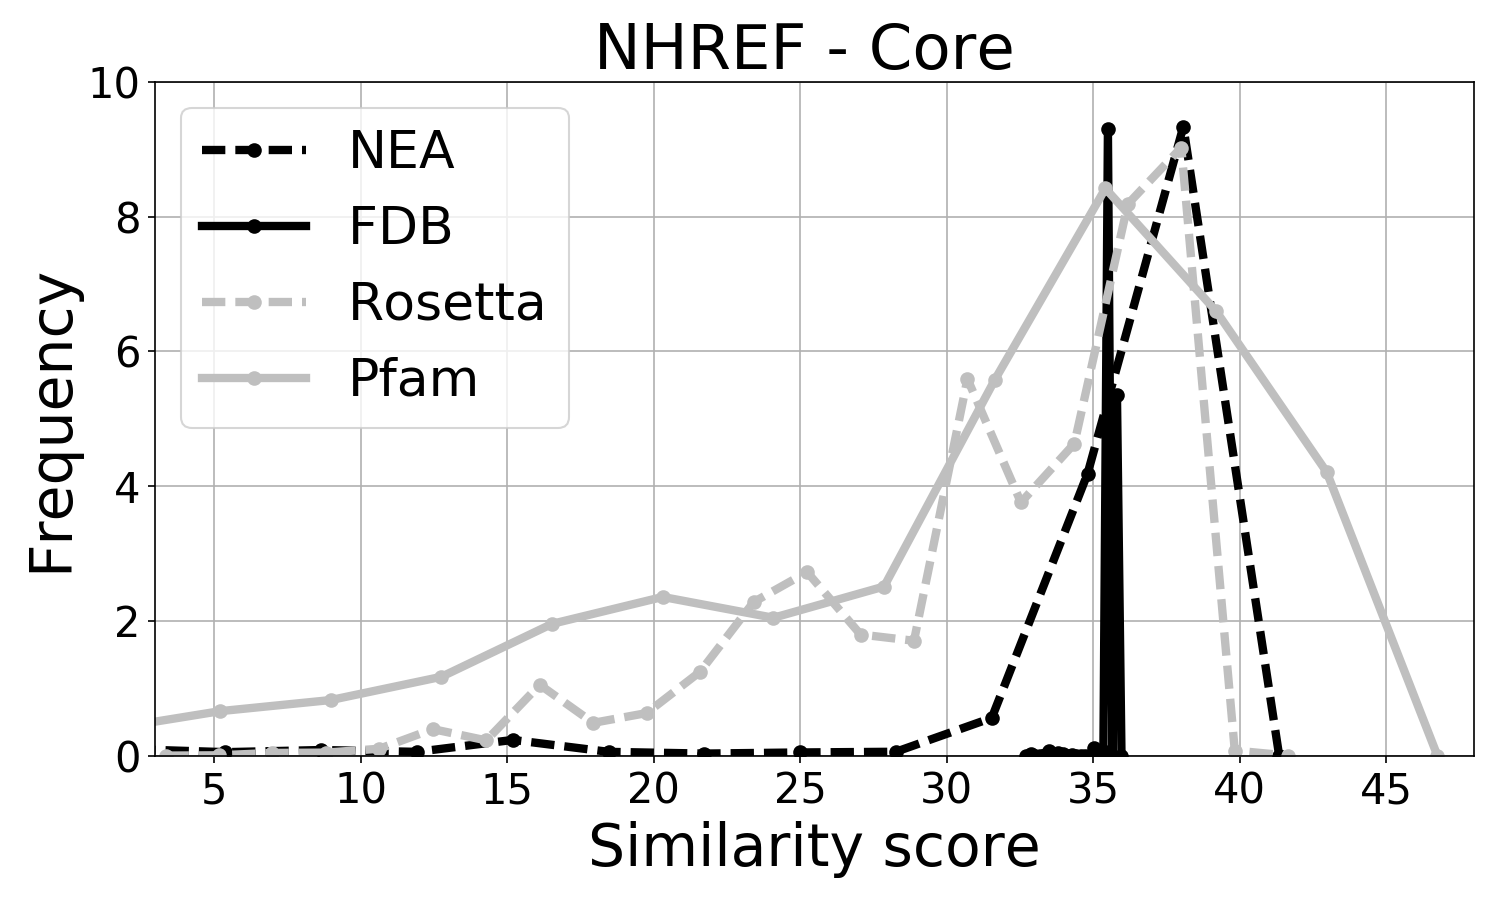
\includegraphics[width=8.4cm]{rapport/resultats/PDZ/graphe/exactGB/1G9O_simil_core.png} \\
       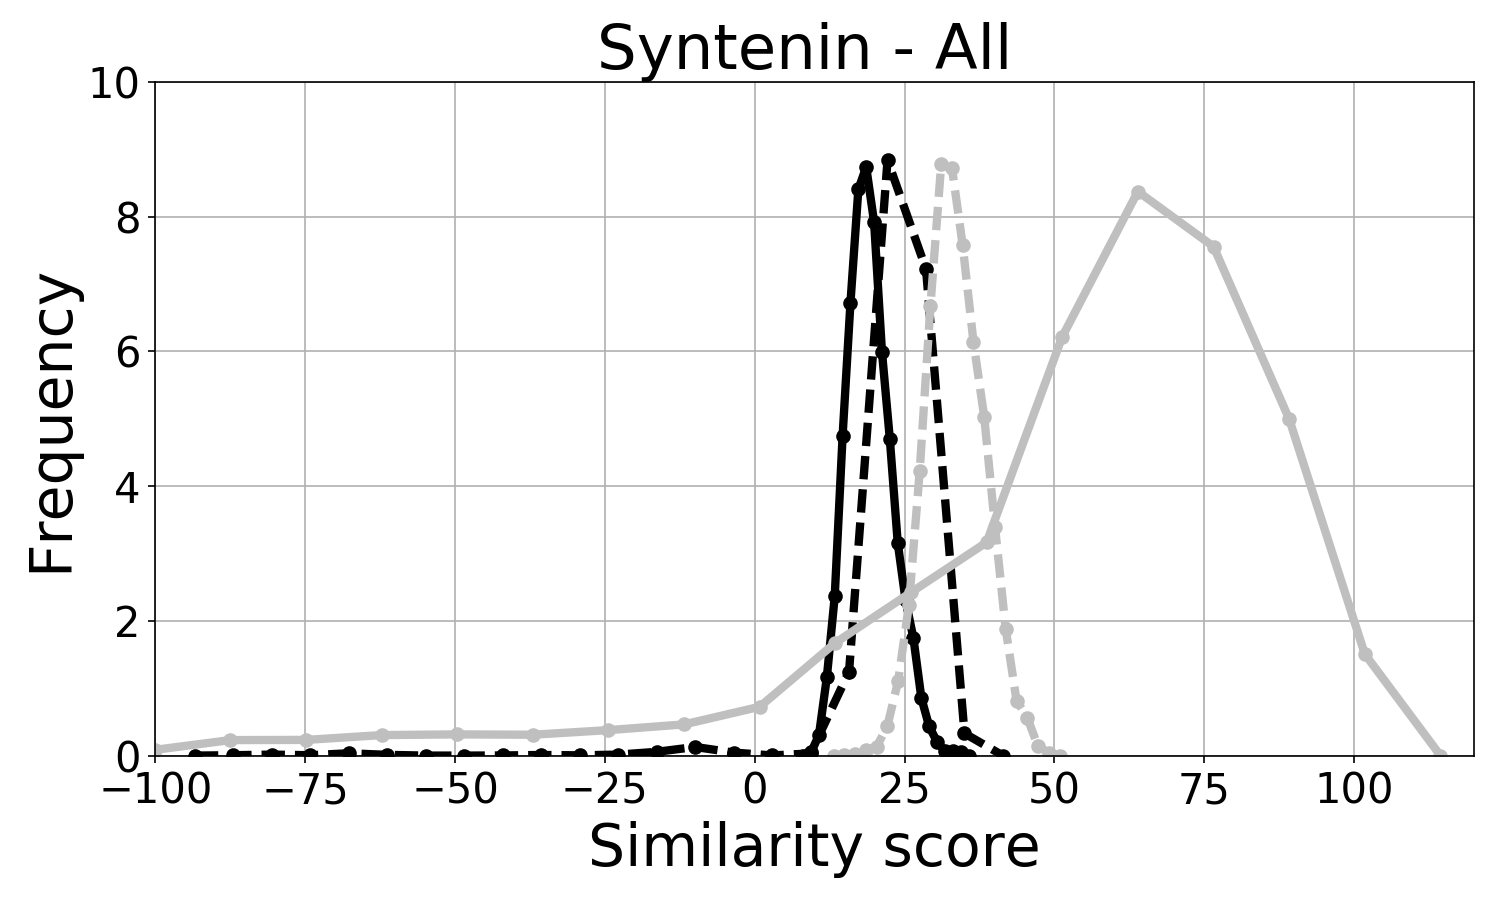
\includegraphics[width=8.4cm]{rapport/resultats/PDZ/graphe/exactGB/1R6J_simil_cut.png} &
       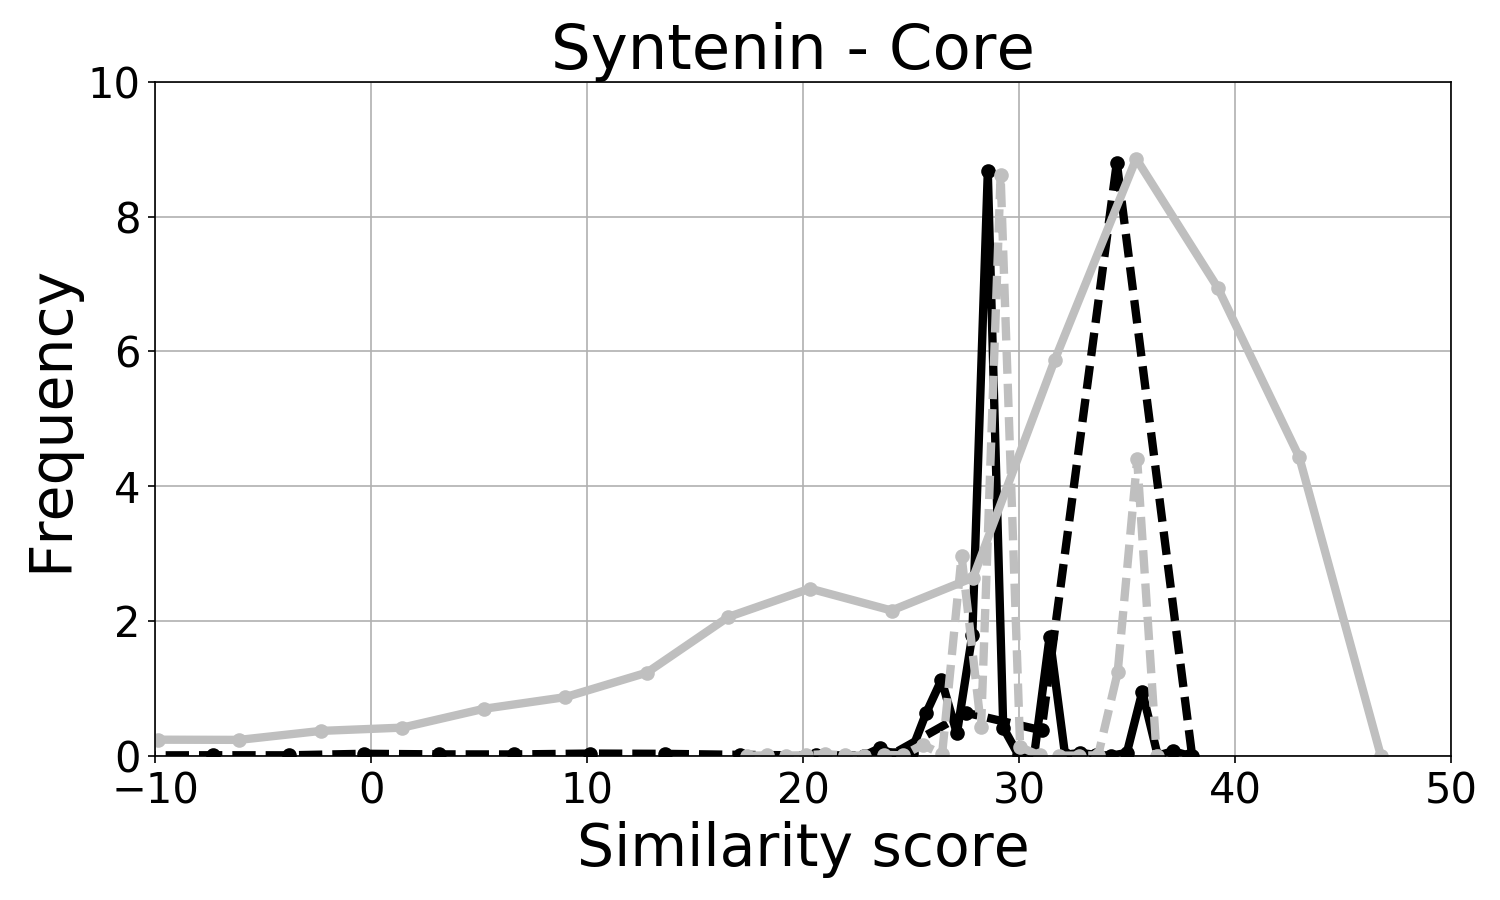
\includegraphics[width=8.4cm]{rapport/resultats/PDZ/graphe/exactGB/1R6J_simil_core.png} \\
       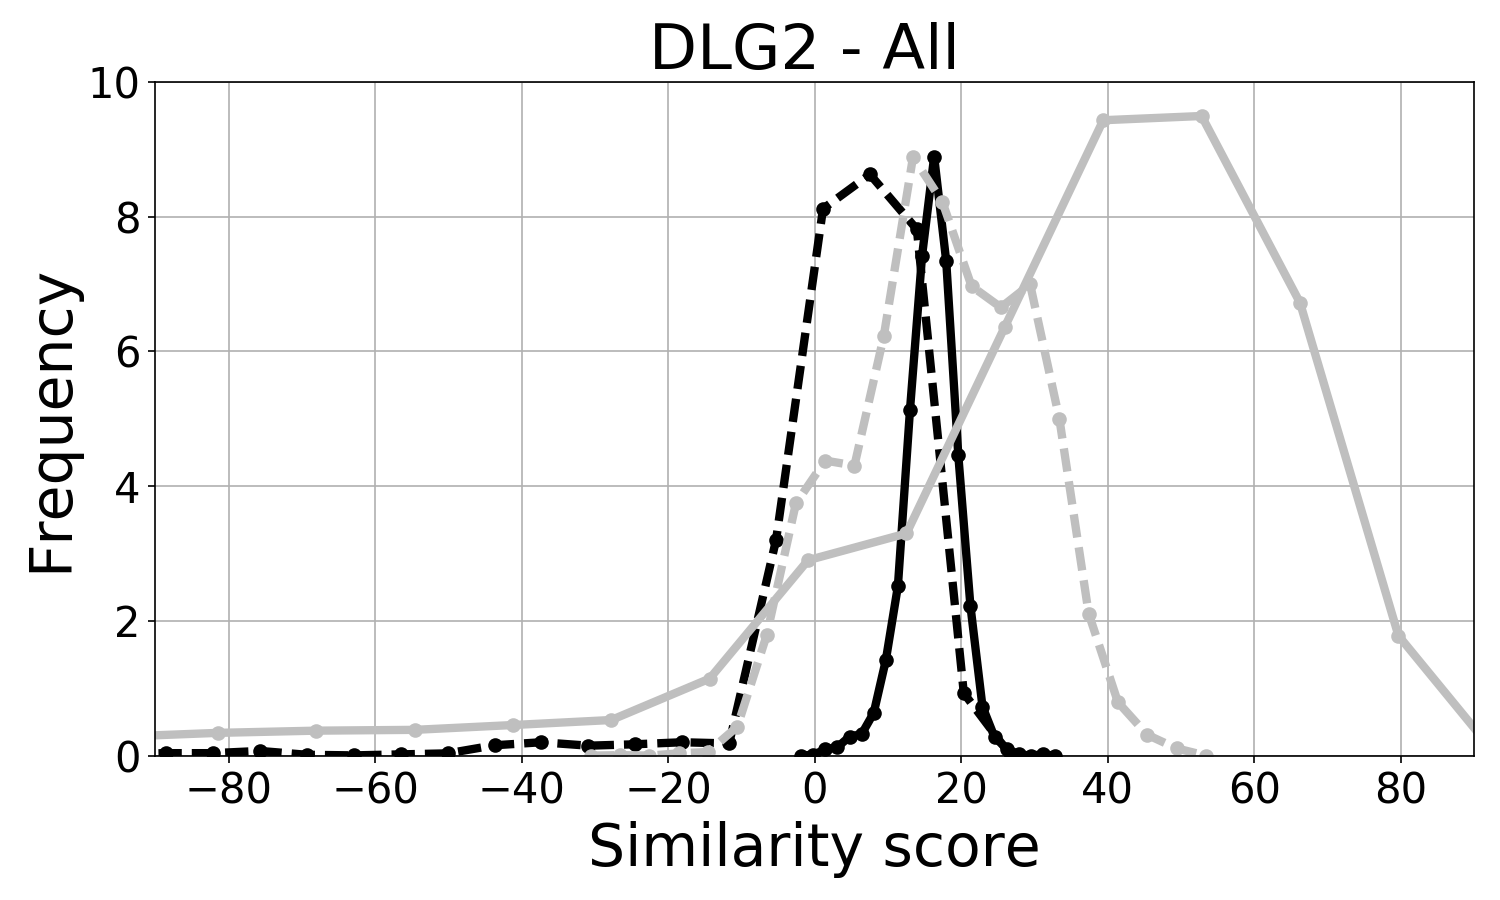
\includegraphics[width=8.4cm]{rapport/resultats/PDZ/graphe/exactGB/2BYG_simil_cut.png} &
       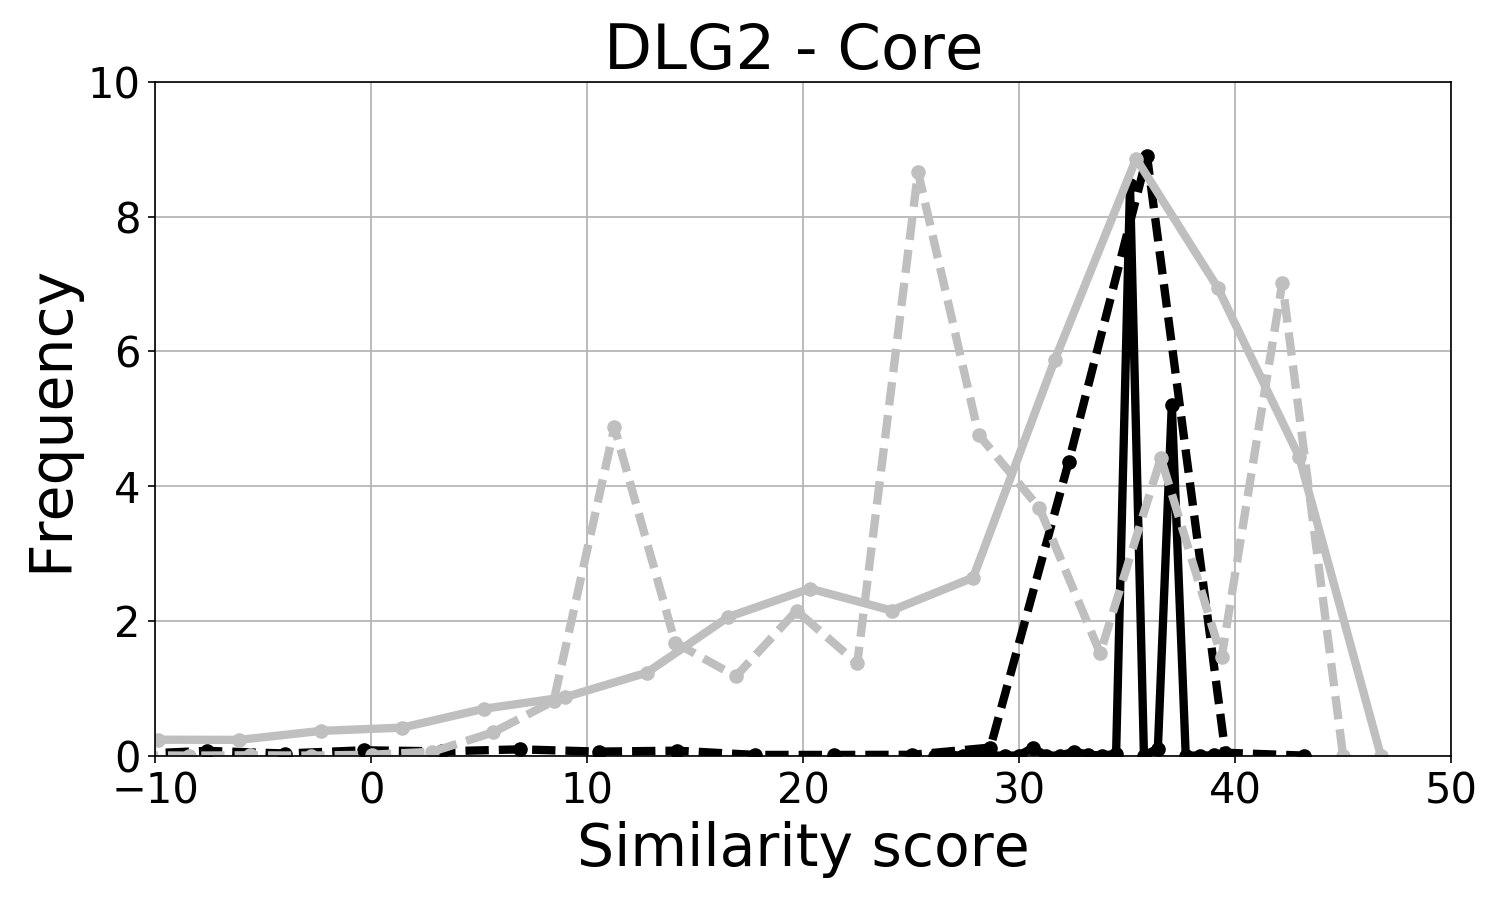
\includegraphics[width=8.4cm]{rapport/resultats/PDZ/graphe/exactGB/2BYG_simil_core.png} \\
     \end{tabular}
\label{graph:Simil_Proteus_PDZ}
   \end{figure}



   \clearpage
   
    \begin{table}[!htbp]
      \centering

      \begin{tabular}{ccccc}

        \toprule
        \toprule
        \multirow{2}{*}{Residues}  & \multicolumn{2}{c}{NEA} & \multicolumn{2}{c}{FDB} \\
        \cmidrule(l{2pt}r{2pt}){2-3} \cmidrule(l{2pt}r{2pt}){4-5}
         & Buried & Exposed & Buried & Exposed \\
        \cmidrule{1-5}

        ALA &   0.00     &  0.00    &   0.00  &   0.00       \\
        CYS &  -0.89     &  -2.57   &  -1.06  &   -1.64      \\
        THR &  -5.31     &  -8.075  &  -4.84  &   -6.68      \\
        SER &  -5.55     &  -6.55   &  -4.45  &   -5.24      \\
        ASP &  -17.26    &  -22.06  &  -14.56 &   -18.82     \\
        GLU &  -16.12    &  -20.68  &  -14.52 &   -18.21     \\
        ASN &  -16.38    &  -20.41  &  -14.02 &   -17.80     \\
        GLN &  -14.00    &  -18.41  &  -13.14 &   -16.61     \\
        HID &   11.21    &  6.95    &  10.85  &   8.13       \\
        HIE &   10.63    &  6.15    &  10.41  &   7.37       \\
        HIP &   15.17    &  10.72   &  12.86  &   10.98      \\
        ARG &  -53.40    &  -57.36  &  -51.37 &   -54.76     \\
        LYS &  -8.20     &  -12.34  &  -8.24  &   -11.35     \\
        ILE &   6.76     &  3.44    &  5.50   &   3.06       \\
        VAL &   0.43     &  -2.19   &  -0.05  &   -1.66      \\
        LEU &   0.52     &  -3.72   &  0.00   &   -2.94      \\
        MET &  -1.61     &  -3.21   &  -2.85  &   -3.09      \\
        PHE &   1.86     &  -2.68   &  0.17   &   -3.18      \\
        TRP &  -0.23     &  -7.67   &  -1.94  &   -5.53      \\
        TYR &  -5.10     &  -10.90  &  -5.91  &   -10.14     \\

        \bottomrule


      \end{tabular}      
      \caption{Les énergies de référence obtenues avec l'optimisation 6 protéines.}
\label{tab:RefEner_groupes}      
    \end{table}



   
\thispagestyle{empty}

\end{document}
 

